\chapter{Governing Equations} \label{ch:gov_eqns}

The governing species transport equations are implemented into a coding structure based on a finite volume discretization. First the integral volume formulation of the species transport equation is derived. Next volumetric source terms for isotopic species, boundary conditions and phase coupling are discussed. Finally, the interfacial area tracking method is derived.

\section{Conservation of species for multi-phase flow}
Consider the fixed control volume for two phase flow show in Figure \ref{fig:gen_control_volume}.

In deriving the conservation of species relation we will first start with the relation for a system with a single phase. Let \textit{C} be the conserved quantity of interest in amount per unit volume and let \textit{F} be the flux, amount per unit area per time passing through the unit normal surface of \textit{V}. If the quantity \textit{C} is being generated in control volume \textit{V} then let its generation rate be denoted by ${C_{V}}$. Equation \ref{eq:gen_species_con_integral_volume} represents the conservation of species in a fixed control volume. 


% Control Volume
\begin{figure}[ht]
  \centering
  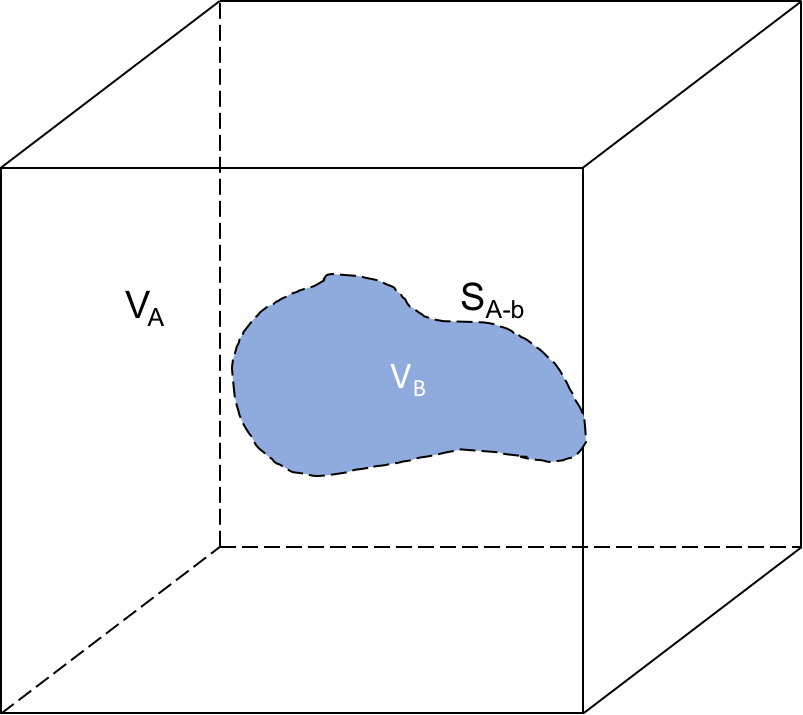
\includegraphics[width=3in]{two_phase_cell_volume.png}\\
  \caption{General control volume.}
  \label{fig:gen_control_volume}
\end{figure} 

% General equation species integral volume
\begin{equation}
	\frac{\partial }{\partial t}\iiint_V C \,dV = -\iint_S n \cdot F \,dS + \iiint_V C_{V} \,dV
	\label{eq:gen_species_con_integral_volume}
\end{equation}

The differential operator in the first term of Equation \ref{eq:gen_species_con_integral_volume} can be brought inside the integral by applying Leibniz integral rule shown below.

% Application of Leibniz rule
\begin{equation}
	\frac{\partial }{\partial t}\iiint_V C \,dV = \iiint_V \frac{\partial C}{\partial t}\,dV
\end{equation}

This simplifies equation \ref{eq:gen_species_con_integral_volume} to 

% Plugging in Leibniz rule to the general equation
\begin{equation}
	 \iiint_V \frac{\partial C}{\partial t}\,dV = -\iint_S n \cdot F \,dS + \iiint_V C_{V} \,dV
	\label{eq:gen_species_con_integral_volume_leibniz}
\end{equation}

Let a phase be a region where \textit{C} is a continuous function and interfaces are surfaces which can introduce discontinuities in \textit{C}. Using Equation \ref{eq:gen_species_con_integral_volume_leibniz}, Leibniz integral rule is applied to the time derivative of each phase volume separately. 

% apply Leibniz rule to volume A
\begin{equation}
	\frac{\partial }{\partial t}\iiint_{V_{A}} C \,dV = \iiint_{V_{A}} \frac{\partial C}{\partial t}\,dV + \iint_{S_{I}} C_{A} n_{I} \cdot v_{I} \,dS
	\label{eq:leibniz_rule_volA}
\end{equation}

% apply Leibniz rule to volume B
\begin{equation}
	\frac{\partial }{\partial t}\iiint_{V_{B}} C \,dV = \iiint_{V_{B}} \frac{\partial C}{\partial t}\,dV - \iint_{S_{I}} C_{B} n_{I} \cdot v_{I} \,dS
	\label{eq:leibniz_rule_volB}
\end{equation}

The last term in Equations \ref{eq:leibniz_rule_volA} and \ref{eq:leibniz_rule_volB} take into account the velocity of the phase interface. In equation, this contribution is subtracted due to the unit normal point in the opposite direction. These two equations can be added together to represent the entire volume. 

% Leibniz rule for vol A, B
\begin{equation}
	 \iiint_V \frac{\partial C}{\partial t}\,dV = -\iint_S n \cdot F \,dS + \iiint_V C_{V} \,dV + \iint_{S_{I}} (C_{A} - C_{B}) n_{I} \cdot v_{I} \,dS
	\label{eq:two_phase_time_term}
\end{equation}

The last term in Equation \ref{eq:two_phase_time_term} is only present when  the interface is moving and \textit{C} is discontinuous. If a source term is present in the interface then the rate of formation per unit area of interface is ${C_{S}}$. 

% combining all terms for a two phase system
\begin{equation}
	 \iiint_V \frac{\partial C}{\partial t}\,dV = -\iint_S n \cdot F \,dS + \iiint_V C_{V} \,dV + \iint_{S_{I}} (C_{A} - C_{B}) n_{I} \cdot v_{I} \,dS + \iint_{S_{I}} C_{S}   \,dS
	\label{eq:two_phase_Intarea_source}
\end{equation}

When more than two phases are present, then the last two terms in Equation \ref{eq:two_phase_Intarea_source} are represented as summations for all phases present. The integral formulation at an interface can also be represented by Equation \ref{eq:alt_integral_surface} \cite{deen2016}.

% representing the source term at an interface
\begin{equation}
	 \iint_S [(F - CV_{I})_{B} - (F - CV_{I})_{A})]\,dS = \iint_S C_{S} \,dS
	\label{eq:alt_integral_surface}
\end{equation}

Where the term $F - CV_{I}$ is the flux relative to the interface. For an arbitrary number of phases, species can be represented as a balance over each phase volume. 

% two-phase volume equation
\begin{equation}
	\iiint_{V} \frac{\partial \alpha_{k}C_{k} }{\partial t}\,dV = -\iint_S n \cdot F_{k} \,dS + \iiint_V \alpha_{k}C_{V,k} \,dV + \iint_{S_{j}} C_{S_{k}} \,dS
	\label{eq:two_phase_species_con_integral_volume}
\end{equation}

These set of equations are the fundamental relations regarding the conservation of species for a multi-phase system. In the case of a multi-component system, these same relations apply, however care must be taken when developing inner species interactions and phase migration. 

% Source terms
\section{Understanding Volumetric Source Terms} \label{source_terms}
To understand the behavior for fission products it is first necessary to understand the source and sink terms for each product of interest. For a general reactor design these terms are represented in Table \ref{tab:volume_source_terms}\cite{houtzeel1967}. 

% table of source and sink terms
\begin{table}[htbp!]
   \caption{\label{tab:volume_source_terms} Source and sink terms for chemical species and elemental isotopes}
   \centering
   \begin{tabular}{l llll}
   \hline
   \textbf{Source/Sink} & \textbf{Mechanisms involved}\\
   \hline 
   Direct from fission & Neutron flux, fission yield \\[1ex]
   Decay from parent atom & Decay constant \\[1ex]
   Transmutation & Neutron flux, microscopic cross-section \\[1ex]
   Phase/material migration & mass transfer, diffusion theory \\[1ex]
   Removal/addition system & Removal efficiency, addition rate \\[1ex]
   Chemical reaction & Reaction rate, thermodynamic equilibrium \\[1ex]
   \hline
   \end{tabular}
\end{table}

To understand the fate of volatile fission products in a MSR we must first derive a rate balance for each species of interest. Molten salts are characterized by having a melting point with reactors operating at temperatures well above liquid temperatures. Because of this, it is assumed that all chemical reaction occurring in the salt happens instantaneously \cite{baes1974}\cite{kedl1972}. This also leads to the next assumption, that the salt is in a pseudo equilibrium state at almost all times. This allows for the calculation of thermophysical properties with the use of Gibbs free energy minimization. 

% Nuclear interactions
\subsection{Nuclear Interactions}
Because volumetric generation rates depend on nuclear reactions, it is important to first understand the mechanisms governing the physical interaction of particles and isotopes. 

% Importance of decay chains
\subsection{Importance of Decay Chains}
Most fission products are atomically unstable and will decay into other elements based on half-lives and decay chains, so these other elements may be created from these decays or separately as direct fission products. This greatly complicates fission product accumulation and accounting, and influences the ultimate disposition. Consider the following decay scheme \cite{kedl1972}:

\begin{equation}
	Fission \space (\gamma_{_{Kr}})\rightarrow Kr \rightarrow Rb \rightarrow Sr \rightarrow Y \rightarrow Zr \rightarrow Nb \rightarrow Mo \rightarrow
\end{equation}

In this scheme Kr is a noble gas, Rb, Sr, Y, Zr are salt seekers, Mo is a noble metal with Nb being either a noble metal or salt seeker depending on redox condition of the carrier salt.  This demonstrates the need to understand fission product decay chains. Likewise, especially for an MSR, an understanding of half-lives relative to the mass transport process cycle times is also needed. For example, if one of the precursors is removed from the system then so will all other elements. However, if removal time is short compared to the half-life then the chain is more likely to proceeded and produce the elements further down the decay chain. 

% Direct from fission
\subsection{Direct Yield from Fission}
Generation rate from fission is a function of neutron flux and fission yield shown in Equation \ref{eq:vol_fission_term} \cite{houtzeel1967}.

\begin{equation}
	rate = \gamma_{i}\Sigma_{f}\phi
	\label{eq:vol_fission_term}
\end{equation}

Where $\gamma_{i}$, $\Sigma_{f}$ and $\phi$ are fission yield, macroscopic fission cross section and neutron flux. The major contribution from this term will be in the liquid salt phase. So, to understand where this term exists one must follow the dissolved salt. If the salt has a tendency to migrate into any process equipment, such as a moderator, for example, then the moderator material will have a fission source term. Fission yields and macroscopic cross sections are not constant, whereby the fission yield is dependent on the nuclear fuel used, and the macroscopic cross section is a function of temperature, material composition and density, and neutron energy. 

% Generation from decay
\subsection{Generation from Decay}
Generation and loss rates due to decay are a function of decay constant and isotope number density, shown in Equation \ref{eq:vol_decay_term} \cite{houtzeel1967}.

\begin{equation}
	rate = + \sum_{j=1}^{N} \lambda_{j\rightarrow i}N_{j} - \sum_{j=1}^{N} \lambda_{i\rightarrow j}N_{i}
	\label{eq:vol_decay_term}
\end{equation}

Where $\lambda$ and $N$ are the decay constant and atomic number densities, respectively. The decay constant is a natural constant and only dependent on the isotope of interest. As noted above, nuclear decay can be both a source and sink term.  If the isotope of interest $i$ is not stable then it will decay into another isotope $j$, making it a sink. Alternatively, if isotope $i$ is being generated from the decay of its parent $j$, then it becomes a source term. 

% Generation from transmutation
\subsection{Generation from Transmutation}
Generation from transmutation is a function of neutron flux, number density and microscopic cross section, as shown in Equation \ref{eq:vol_trans_term} \cite{houtzeel1967}.

\begin{equation}
	rate = + \sum_{j=1}^{N} \sigma_{j\rightarrow i}N_{j}\phi - \sum_{j=1}^{N} \sigma_{i\rightarrow j}N_{i}\phi
	\label{eq:vol_trans_term}
\end{equation}

Where $\sigma_{i\rightarrow j}$, $N_{i}$, and $\phi$ are microscopic cross section for the transmutation of isotope $i$ into $j$, or vice versa, atomic number density and neutron flux.  Similar to the generation from decay, a summation is needed to account for all isotopes that can transmute into isotope $i$ or transmute from isotope $i$ into another isotope $j$. Note that the macroscopic cross section is the product of a number density and a microscopic cross section, thus, microscopic or macroscopic cross sections are functions of temperature and neutron energy.

% Removal rate
\subsection{System Removal and Addition}
This term is dependent on the MSR design and must be evaluated for each design case. A simple example of removal rate from salt is shown in Equation \ref{eq:vol_removal_term}.

\begin{equation}
	rate = S_{eff}\dot{M}_{i}
	\label{eq:vol_removal_term}
\end{equation}

Where $S_{eff}$ and $\dot{M}_{i}$ are system removal efficiency and mass flow rate of species $i$. In general, the system removal coefficient can be defined in a number of ways ($i.e.,$ volumetric or mass flow rate) so the appropriate conversions must be taken.  

% Boundary conditions
\section{Boundary Conditions and Phase Coupling}
In this work, boundary conditions are defined as the mathematical formulation of physical phenomena that occur across phase/material boundaries in the solution domain. This can include phase migration ($i.e.,$ species dissolving or absorbing out of solution) and material migration, such as species plating out to a solid surface and or material migrating from liquid to solid surfaces.  For any boundary (liquid-gas, liquid-solid, solid-gas), Equation \ref{eq:alt_integral_surface} is valid. In the absence of bulk movement across the boundary the normal component of the velocity in either phase is equal to the normal component of the interfacial velocity \cite{deen2016}. This simplifies the flux term \textit{F} to only the diffusive flux component. 



\begin{equation}
	J_{in_{2}} - J_{in_{1}} = C_{S_{in}}
\end{equation}

Here, $J$ is the flux from either side of the surface and $C_{S_{in}}$ is a surface generation rate. If there are no surface source terms at the surface then the two diffusive fluxes are equal to one another. 

%\subsection{Diffusion fluxes}

For binary and mixtures, Fick's Law can be used when determining the species diffusive flux. Fick's Law describes the flux as a relation of a diffusion coefficient multiplied by the gradient of species concentration across a spatial length shown in Table \ref{tab:ficks_law} \cite{deen2016}.

For multi-component mixtures a pseudo-binary approximation can be used. In the assumption, a mixture of species is dissolved in a mixture where their concentrations dilute and it is assumed that they only interact with the solvent in which they are dissolved.

% two-phase interfaces
\subsection{Two-phase Interface}

In two-phase systems, the transfer of a species will continue along an interface until an equilibrium is reached. One common mechanism which describes this process is commonly known as two-film theory or two-resistance theory. Transport across an interface can be broken down into three steps.

\vspace{12.7mm} %5mm vertical space

 % table of ficks law for difference reference velocities. 
\begin{table}[htbp!]
   \caption{\label{tab:ficks_law} Fick's Law for various units}
   \centering
   \begin{tabular}{l ll}
   \hline
   \textbf{Reference velocity} & \textbf{Diffusive flux}\\
   \hline 
   ${\textbf{v}_{mass}}$ & $J =  -\rho D_{AB} \nabla \omega_{A}$ \\[1ex]
   ${\textbf{v}_{molar}}$ & $J =  -C D_{AB} \nabla x_{A}$ \\[1ex]
   \hline
   \end{tabular}
\end{table}

\newpage

\begin{enumerate}
	\item Transport of species from bulk of phase 1 to phase 1 interface
	\item Transport across the interface
	\item Transport from phase 2 interface to phase 2 bulk
\end{enumerate}

The two-resistance theory assumes that the rate for the overall transfer is determined from rate at which a species diffused from bulk to interface and from interface to bulk. In other words, the resistance transport across an interface in negligible \cite{wilson1969}. 

At phase interfaces, a local equilibrium does not imply equal concentrations on both sides of the interface, as shown in Figure \ref{fig:general_phase_interface}. The two concentration are however, related to one another by the partition coefficient \cite{deen2016}. The patrician coefficient $K_{P,i}$ is calculated based on the relative solubility of species i in the two phases. For a liquid-gas interface, Henry's law can be used and is shown in Equation \ref{eq:partition_coefficient}.

 \begin{equation}
	C_{i,1} = K_{P,i}C_{i,2}
	\label{eq:partition_coefficient}
\end{equation}

\begin{figure}[ht]
  \centering
  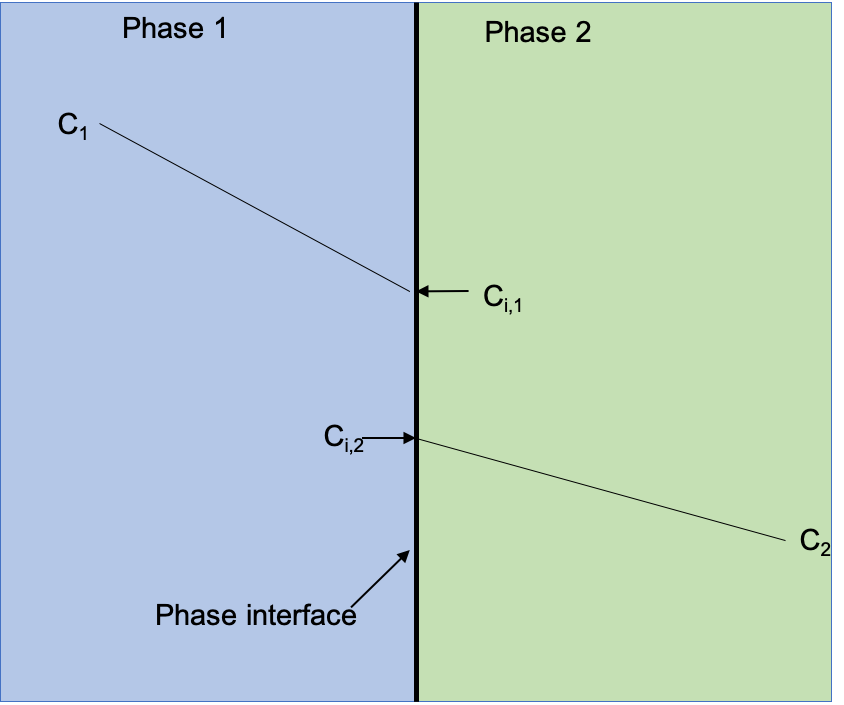
\includegraphics[width=3.2in]{images/general_phase_interface.png}\\
  \caption{Concentration profile across an interface}
  \label{fig:general_phase_interface}
\end{figure} 

\newpage

In situations where there is no phase change (i.e. no bulk flow across the interface) a convection boundary condition can be applied \cite{deen2016}. 

 \begin{equation}
	J_{in,2} =J_{in,1} = k_{2}(C_{in,2} - C_{bulk}) = k_{1}(C_{bulk} - C_{in,1})
	\label{eq:convection_boundary_condition}
\end{equation}

Equation \ref{eq:convection_boundary_condition} states that the flux across a boundary is proportional to the difference in concentration between the bulk fluid in phase k and the interface multiplied by the mass transfer coefficient $k_{ci}$. It is important to note that the driving force for species transport is the concentration only in the phase in question. Instead of using individual mass transfer coefficients, Equation \ref{eq:convection_boundary_condition} can also be represented using overall mass transfer coefficients $K_{i}$ \cite{bird2006}.

 \begin{equation}
	J_{in,2} =J_{in,1} = K_{2}(C_{e,2} - C_{bulk}) = K_{1}(C_{bulk} - C_{e,1})
	\label{eq:overall_convection_boundary_condition}
\end{equation}

$C_{e,2}$ and $C_{e,1}$ represent the equilibrium concentration in either phase. Using Equations \ref{eq:partition_coefficient}, \ref{eq:convection_boundary_condition} and  \ref{eq:overall_convection_boundary_condition} the following expression is obtained to relation single-phase and two-phase mass transfer coefficients for a liquid-gas system.

\begin{equation}
	\frac{1}{K_{G}} = \frac{1}{k_{G}} + \frac{m}{k_{L}}
	\label{eq:gas_phase_resistance}
\end{equation}

\begin{equation}
	\frac{1}{K_{L}} = \frac{1}{k_{L}} + \frac{1}{mk_{G}}
	\label{eq:liq_phase_resistance}
\end{equation}

Where \textit{m} is derived using Henry's law. For processes in which $ m >> 1$, $ \frac{1}{mk_{G}} $ approaches zero and mass transfer is liquid-phase controlled. On the other hand, if $ m << 1$, $ \frac{1}{mk_{G}}$ becomes very large, making the system gas-phase controlled. For systems which obey Henry's Law, the over all mass transfer coefficient can be represented by

 \begin{equation}
	\frac{1}{K_{L}} = \frac{1}{k_{L}} + \frac{HRT}{k_{G}}
\end{equation}

Therefore, if the Henry's law constant is very small i.e. the chemical species is sparsely  soluble in the liquid, then the contribution from $k_{G}$ is small and can be ignored. 

For a species i initially in the gas phase or gas bubbles, the rate at which i migrates into the liquid phase is modeled using Equation \ref{eq:gas_side_coupling}, where $a$ and $V$ are interfacial area and volume.

\begin{equation}
    \frac{\partial C_{i}^{g}}{\partial t} = \frac{Ka}{V}\Big[C_{i}^{l}  - C_{i}^{*}\Big]
    \label{eq:gas_side_coupling}
\end{equation}

The equilibrium concentration $C_{i}^{*}$ in the liquid is determined using Henry's law. In the case for a gas that is insoluble in the liquid, $H \rightarrow 0$ meaning that the only changed in concentration is due to migration from the liquid side. Because the fluxes are equal across both boundary's, the liquid side phase migration is governed by Equation \ref{eq:liq_side_coupling}.

\begin{equation}
    \frac{\partial C_{i}^{l}}{\partial t} = \frac{Ka}{V}\Big[C_{i}^{*} - C_{i}^{l}\Big]
    \label{eq:liq_side_coupling}
\end{equation}

In the case of a gas born inside of a liquid solution Equation \ref{eq:liq_side_coupling} governs its migration into the bulk gas phase. If the gas is insoluble in the liquid then again $H \rightarrow 0$ and its migration rate is governed by the concentration in the liquid and the mass transfer coefficient. 


% Mass transfer coefficients
\section{Mass Transfer Coefficients}
Mass transfer coefficients are of great importance to the understanding of interface mass transport. There are many different ways in which mass transfer coefficients can be derived. For simple situations, mass transfer coefficients can be derived using first principles \cite{perry2007}. However, in industrial applications most of these coefficients are empirically defined from experimental data. In many situations, a number of corrections may exist and one must be careful to use the appropriate coefficients. The Perry's Chemical Engineers' Handbook \cite{perry2007} states the following heuristics to aid in choosing the appropriate coefficients.

\begin{enumerate}
	\item Mass-transfer coefficients are derived from models. The must be employed in a similar model. For instance, if $k$ is defined for a difference in concentration, it should only be used with an arithmetic concentration difference. 
	\item Semi-empirical correlations are often better than purely empirical or purely theoretical 
	\item Correlations with wide data sets
	\item The analyogy between heat and mass transfers holds over wider ranges than mass and momentum transfer. 
	\item More recent data is preferred over older data. 
	\item Complicated geometries requires the use of volumetric mass transfer coefficients. 
\end{enumerate}

\subsection{Stagnant-film Model}
This approach assumes the steady state unidirectional diffusion through a stagnate film adjacent to the surface. The process of mass transfer is driven by molecular diffusion across the film thickness. Film thickness depends on depends on the Reynolds and Schmidt number. Using Fick's law, the mass transfer coefficient is proportional to the the diffusion coefficient over the film thickness \cite{perry2007}. For example, the liquid side mass transfer coefficient is represented by Equation \ref{eq:liq_side_sag_film}

\begin{equation}
	k_{L} = \frac{D}{\delta_{L}}
	\label{eq:liq_side_sag_film}
\end{equation}

\subsection{Penetration theory}
Penetration model was first proposed by R. Higbie in 1935 \cite{asano2006} to predict the mass transfer in a packed tower \cite{perry2007}. In this model, liquid flows across packing in laminar flow and is remixed in a transient fashion as you move across the packing material. The timed average mass transfer coefficient is given by Equation \ref{eq:liq_side_penetration_theory}.

\begin{equation}
	k_{L} = 2 \sqrt{\frac{D_{L}}{\pi t}}
	\label{eq:liq_side_penetration_theory}
\end{equation}

Where $t$ is the contact time which is not known in many cases.

\subsection{Surface Renewal Theory}
Danckwerts extended Penetration theory to what is known as Surface renewal theory \cite{perry2007}. Surface renewal theory allows for the continuous replacement of the liquid to the interior surface. The liquid is exposed to gas for for finite lengths of time before being replace with fresh fluid. Equation \ref{eq:liq_side_surface_theory} represents the mass transfer coefficient. 

\begin{equation}
	k_{L} = \sqrt{D_{L} s}
	\label{eq:liq_side_surface_theory}
\end{equation}

Where $s$ is the fraction rate of surface renewal. 

\subsection{Mass transfer correlations}
The rate of mass transfer is often described by the Sherwood number which is analogous to the Nusselt number for heat transfer. The Sherwood number ($Sh$) is a dimensionless number defined as the convective mass flux over the diffusion flux at the interface. 

% Sherwood number
\begin{equation}
	Sh = \frac{h}{D/L} = \frac{\text{Convective mass transfer}}{\text{Diffusive mass transfer}}
	\label{eq:sherwood_number}
\end{equation}

In terms of dimensionless numbers, the Sherwood number can also be defined as a function of Reynolds number ($Re$) and Schmidt number ($Sc$). The Reynolds number represents the inertial forces over the viscus forces, with the Schmidt number corresponding to the viscus diffusion rate over the mass diffusion rate. 

% Reynolds number
\begin{equation}
	Re = \frac{\rho v L}{\mu} = \frac{\text{Inertial forces}}{\text{Viscus forces}}
	\label{eq:reynolds_number}
\end{equation}

% Schmidt number
\begin{equation}
	Sc = \frac{\mu}{\rho D} = \frac{\text{Viscus diffusion}}{\text{Mass diffusion}}
	\label{eq:schmidt_number}
\end{equation}

There are many correlations for calculating the Sherwood number, will all being problem specific. Anther aspect to take into consideration is the fact that both Equations \ref{eq:sherwood_number} and \ref{eq:schmidt_number} require the diffusion coefficient. For single small bubbles (modeled as solid spheres) of gas in dilute liquid systems the the Sherwood correlation is given by \cite{perry2007}

% Small bubble sherwood number
\begin{equation}
	Sh = \frac{k d_{b}}{D} = 1.0(Re Sc)^{1/3} \qquad d_{b} < 0.1\text{cm}
	\label{eq:mass_transfer_corelation_small_bub}
\end{equation}

% Small bubble sherwood number
\begin{equation}
	Sh = \frac{k d_{b}}{D} = 1.13(Re Sc)^{1/2} \qquad d_{b} >0.5\text{cm}
	\label{eq:mass_transfer_corelation_big_bub}
\end{equation}

During MSRE operations, the bubble size rang considered was 0.0127cm - 0.0508 cm \cite{engel1971}, well in the range of Equation \ref{eq:mass_transfer_corelation_small_bub}. 

% Interfacial area tracking 
\section{Interfacial Area Tracking}

The interfacial area plays a critical role in the calculation of species migration between two phases. These areas can remain relatively constant or (in the case of liquid-gas phase) be highly variable. Take for instance the diffusion of gas initially dissolved in the liquid phase into a rising bubble. As the the bubble rises the dissolved gas migrates into the bubble increases the number of moles the bubble contains. Also, as the bubble rises the effect of hydrostatic pressure diminishes. Therefor, as the bubble rises, its interfacial area increases. This is because pressure is inversely correlated to gas volume, so as the bubbles surrounding pressure decreases, its volume increases. For mass, as the amount of gas inside of the bubble increases from mass transfer, the bubble volume increases.

Equations of state (EOS) describe the relations of four variables have on a gas phase substance. These include: pressure, temperature, volume and mass or moles. One of the most widely utilized EOS is the ideal gas law, shown in Equation \ref{eq:ideal_gas_law}. The ideal gas law is valid for systems of low pressure, high specific volume, and no molecular interactions. There are other EOS which one can use, such as Van der Waals and Peng-Robinson which account for molecular interactions and other situations for which the ideal gas law falls short. In this report, the ideal gas law is chosen for its simplicity and relative validity. 

For a bubble suspended in solution, its volume is calculated using the ideal gas law.

% Ideal gas law
 \begin{equation}
	PV = nRT
	\label{eq:ideal_gas_law}
\end{equation}

$P$ is pressure, $V$ is volume, $n$ is moles, $T$ is temperature, and $R$ is the universal gas constant. With all of the properties just mentioned to be represented as pertaining to the bubble i.e. T, P are the temperature and pressure inside the bubble.

Assuming the bubble is small and of spherical shape, the volume volume is calculated by,
 
% volume of sphere
 \begin{equation}
	V = \frac{\pi d^{3}}{6}
	\label{eq:vol_of_sphere}
\end{equation}

Where d is bubble diameter. Plugging into the idea gas law, 

 \begin{equation}
	P \frac{\pi d^{3}}{6} = nRT
	\label{eq:vol_of_bubble}
\end{equation}

For static bubbles for which the forces are uniform across its surface, the Young-Laplace Equation \ref{eq:young-laplace} is used to calculate the pressure inside of the gas bubble \cite{deen2016}. 

% Young-Laplace 
 \begin{equation}
 	P_{b} = P_{l} + \frac{4 \sigma_{l}}{d}
	\label{eq:young-laplace}
\end{equation}

Where $P_{b}$, $P_{l}$, $\sigma_{l}$ and $d$ are bubble pressure, liquid pressure, surface tension, and bubble diameter. The bubbles are considered to be in thermal equilibrium with the surrounding fluid, meaning $T_{b} = T_{l}$.  Plugging in Equation \ref{eq:young-laplace} into \ref{eq:vol_of_bubble} yields.

% bubble model
 \begin{equation}
 	\bigg[P_{l} + \frac{4 \sigma_{l}}{d} \bigg] \frac{\pi d^{3}}{6} = nRT_{l}
	\label{eq:bubble_model}
\end{equation}

In Equation \ref{eq:bubble_model} we are solving for bubble diameter. To do this, liquid pressure, temperature, and surface tension are acquired from the CTF solution domain. In order to calculate the number of moles a single gas bubble, a mole balance is preformed across each finite cell volume. Figure \ref{fig:bubbles_in_cell} shows a distribution of bubbles in a cell volume. 

% bubbles in cell
\begin{figure}[ht]
  \centering
  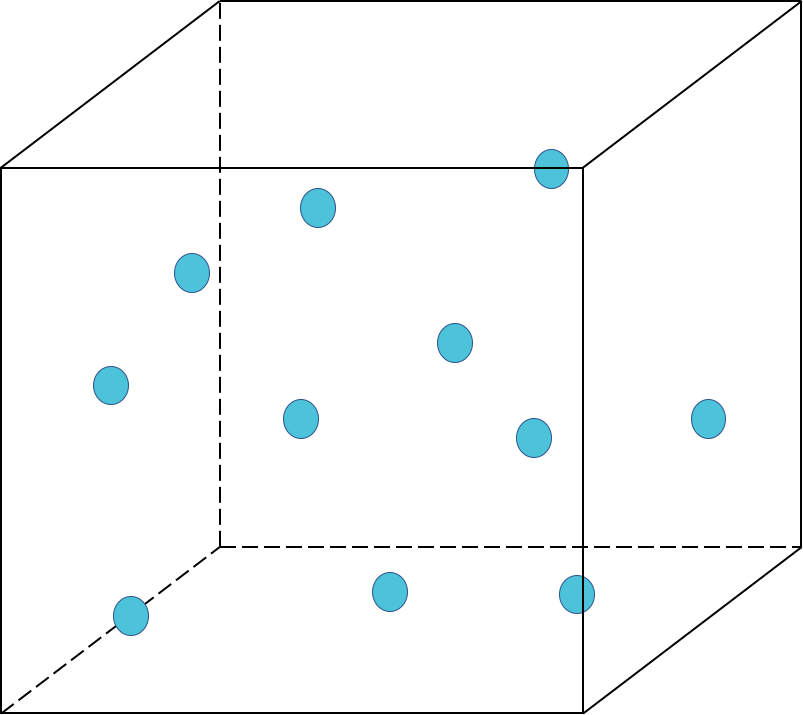
\includegraphics[width=2in]{bubbles_in_cell.png}\\
  \caption{Bubbles dispersed in cell volume.}
  \label{fig:bubbles_in_cell}
\end{figure} 

The number of moles, represented by n, is the summation of all chemical/elemental species in a the bubble. For a system for which we are trying to remove Xenon gas using Helium as our sparging gas, n could be a collection of Helium and Xenon gas. The number of moles in a single bubble is calculated by dividing the total moles of gas in the cell by the number of bubbles. 

 \begin{equation}
 	n_{bubble} = \frac{1}{\# of bubbles} \sum_{j=1}^{k} n_{j}
\end{equation}

The number of bubbles determined from a species transport solve. Because the void faction in the MSRE is so low ($>$1.0 \%) \cite{engel1971}, bubble interactions are neglected. Bubble diameter is solved using the assumption what all bubbles in the cell volume are the same size. 

Two solution methods are employed to solve for bubble diameter. The first involves solving the non-linear Equation \ref{eq:bubble_model} using Newtons Method, which will be discussed later. The second involves making the assumption $P_{b} \approx P_{l}$, this allows for the direct calculation of bubble diameter. 

\begin{equation}
 	D = \bigg(\frac{6nRT_{l}}{\pi P_{l}} \bigg)^{1/3}
	\label{eq:direct_bubble_solve}
\end{equation}

To justify this assumption, the contribution of bubble pressure due to surface tension bust be low. Looking at Equation \ref{eq:young-laplace},  $ 4\sigma_{l}/d \rightarrow \infty$ as $d \rightarrow 0$. As the bubble gets smaller, the contribution from surface tension increases. The range of bubble sizes considered in the MSRE was between $0.0127 - 0.0508$ cm \cite{engel1971}. Figure \ref{fig:pressure_contribution_of_surface_tension} shows the contribution of surface tension to the bubble pressure for a range of bubbles considered in the MSRE. 

\begin{figure}[ht]
  \centering
  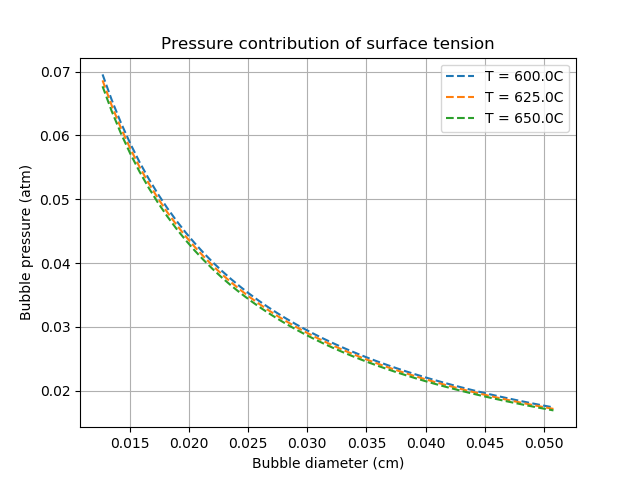
\includegraphics[width=4.5in]{pressure_contribution_of_surface_tension.png}\\
  \caption{Pressure contribution of surface tension.}
  \label{fig:pressure_contribution_of_surface_tension}
\end{figure} 

From Figure \ref{fig:pressure_contribution_of_surface_tension} as expected the contribution from surface tension is highest for smaller bubbles. As temperature increases surface tension slightly decreases leading to a smaller pressure contribution. For a system pressure of 1 and 2 atm, the maximum contribution to the bubble pressure would be 6.54\% and 3.38\% respectively. 

\subsection{Boundary Conditions}\label{ch:bubble_BC}
There are a number of boundary conditions required to solve the interfacial area. These conditions include inlet: temperature, pressure, gas molar flow rate and bubble diameter. Together temperature, pressure, and bubble diameter are utilized in calculating the number of moles in a single bubble by rearranging equation \ref{eq:direct_bubble_solve}. The number of bubbles is calculated by dividing the molar flow rate of gas being injected by the number of moles in a single bubble. 

Gas removal is accomplished by defining a bubble removal efficiency ($S_{eff}$) at the removal location. For gas phase species $i$, the mass flow rate entering the cell is calculated via the flux entering the cell multiplied by the face surface area. The resulting amount of species $i$ exiting the system is then calculated using Equation \ref{eq:vol_removal_term}.












